\documentclass[runningheads]{llncs}
\usepackage{graphicx}
\usepackage{tabularx}

\begin{document}

\title{COMP 472 Project 1 \\ Heuristic Search: Indonesian Dot Puzzle}

\author{Matteo Esposito\inst{1} \and
Matthew Liu\inst{2} \and
Kabir Soni\inst{3}}

\authorrunning{M. Esposito et al.}

\institute{40024121 \email{matteoesposito97@gmail.com} \and
40029238 \email{matthew.jx.liu@gmail.com} \and
40033019 \email{kabirsoni524@gmail.com}}

\maketitle   

\section{Introduction \& Technical Details}

This project was developed using python 3.7.4 64-bit (conda).

\subsection{Files}

The file structure of our project is as follows:

\begin{table}
    \centering
    \caption{Files in project 1}\label{tab0}
    \begin{tabularx}{\textwidth}{|l|l|X|}
        \hline
        \textbf{Directory} & \textbf{Filename} & \textbf{Usage} \\ \hline
        \verb|out_dfs/| & * & Search and solution files for dfs \\ \hline
        \verb|out_bfs/| & * & Search and solution files for bfs \\ \hline
        \verb|out_a_star/| & * & Search and solution files for $A^{*}$ \\ \hline
        \verb|src/| & \verb|input_parser.py| & Input parsing functions, used to cast and convert input data into readable format \\ \hline
        & \verb|board.py| & Board class, used to represent the current puzzle\\ \hline
        & \verb|node.py| & Node class, used in all search algorithm and traversals \\ \hline
        & \verb|dfs.py| & Recursive Limited Depth-First Search algorithm implementation script \\ \hline
        & \verb|bfs.py| & Recursive Best-First Search algorithm implementation script \\ \hline
        & \verb|astar.py| & Recursive and iterative Algorithm $A^{*}$ implementation script \\ \hline
    \end{tabularx}
\end{table}

\subsection{Packages}

We used a total of 7 packages in our project, 5 existing, along with our 2 internal packages (board and node). 

\begin{enumerate}
    \item Existing 
    \begin{itemize}
        \item \verb|shutil| and \verb|os|: Folder and file management in the creation and deletion of output folders for our search and solution files. 
        \item \verb|time|: Runtime output. 
        \item \verb|math|: Updating and calculation of $h$ values (heuristic).
        \item \verb|copy|: Used to create deep copies of parent node when creating child nodes in the \verb|Board.touch()| method.
    \end{itemize}
    \item Internal
    \begin{itemize}
        \item \verb|board|: Class used to represent the puzzle 
        \item \verb|node|: Class that is used to represent the nodes in the tree traversal of all puzzle states involved in the search algorithms.
    \end{itemize}
\end{enumerate}

\subsection{Board and Node Classes}

The board class will take as input the puzzle in the form of a nested list, where each sublist is a row in the dot puzzle provided. The puzzle is converted into a nested list with the help of the \verb|parse()| method of the \verb|input_parser.py| script. It will then allow the search algorithms to call the goal test function to allow the search to terminate, as well as the print grid and touch methods to allow for well formatted printing of the puzzle and child node generation.

The node class will store the current move associated with the resulting puzzle, the puzzle itself (attribute 'state'), the node's parent puzzle. In the non-dfs cases, attributes g, h and f will also be used (cost, heuristic and evaluation function values) to help with the informed searches.

\section{Heuristic}

\textbf{Matthew and Kabir}

\section{Difficulties}

\paragraph{Limited DFS}
Since this was the first algorithm to be implemented, typical difficulties that come with the start of a new project arose (such as project organisation \& strong theoretical understanding of algorithms to be used). These were mainly design issues. Since object-oriented design was a priority, we had to spend some time figuring out how exactly to structure the classes that would be involved in the project. We eventually chose to create a class for the puzzle (Board) and for the nodes which would be later used in the tree-traversal that we end up implementing here.
\paragraph{Best-First Search} blabla
\paragraph{Algorithm $A^{*}$} blabla

\section{Result \& Experiment Analysis}

\underline{Note:} To ensure consistency, all 3 search algorithms were tested on the same 3 sets of inputs as follows:

\begingroup\makeatletter\def\@currenvir{verbatim}
\verbatim
    2 4 100 1001
    3 7 100 111001011
    4 15 10 1010010111001010
\end{verbatim}

\subsection{Limited Depth-First Search}

\begin{table}
    \centering
    \caption{Limited dfs runtimes as a function of the puzzle characteristics}\label{tab1}
    \begin{tabular}{|c|c|c|c|}
        \hline
        \textbf{Puzzle size} & \textbf{Max depth} & \textbf{Runtime} & \textbf{Average memory used} \\
        \hline
        2x2 & 4 & $\sim$ 0.5 seconds & 36.5MiB \\ \hline
        3x3 & 7 & $\sim$ 31 seconds & 36.5MiB \\ \hline
        4x4 & 15 & $\sim$ 52 seconds & 36.5MiB \\ \hline
    \end{tabular}
\end{table}

Compared to the other, informed search algorithms, we expect limited dfs to be the worst performer from a memory usage and time standpoint due to its uninformed nature. This search is also not complete, in that it is not guaranteed to find a solution. Since it is an exhaustive, recursive and stack based search, given branching factor $b$ and depth limit $l$, we have a time complexity of $O(b^l)$ and a space complexity of $O(bl)$. \cite{ref_2}

Using the \verb|memory-profiler| module, which monitors memory consumption of a process \cite{ref_1}, we were able to generate memory usage charts of each of our serach algorithms. We notice that after the initial linear increase in memory usage (due to the I/O and parsing methods prior to the recursive dfs call), we have an average memory usage of 36.5MiB per call of our recursive serach algorithm. (See Appendix A)

\subsection{Best-First Search}

\textbf{Matthew and Kabir}

\subsection{Algorithm $A^{*}$}

\textbf{Matthew and Kabir}

\newpage
\section{Team Responsibilities}

Due to there being three search algorithms that needed to be implemented and we are a group of three, we decided to take on an algorithm each. The breakdown of tasks were as follows:

\begin{enumerate}
    \item Matteo Esposito
    \begin{itemize}
        \item Input parsing functionality
        \item Node \& board class
        \item Limited Depth-First Search
    \end{itemize}
    \item Kabir Soni
    \begin{itemize}
        \item Best-First Search
    \end{itemize}
    \item Matthew Liu
    \begin{itemize}
        \item Board class
        \item Algorithm $A^{*}$
    \end{itemize}
\end{enumerate}

% \noindent Displayed equations are centered and set on a separate
% line.
% \begin{equation}
% x + y = z
% \end{equation}
% Please try to avoid rasterized images for line-art diagrams and
% schemas. Whenever possible, use vector graphics instead (see
% Fig.~\ref{fig1}).

% \begin{figure}
% 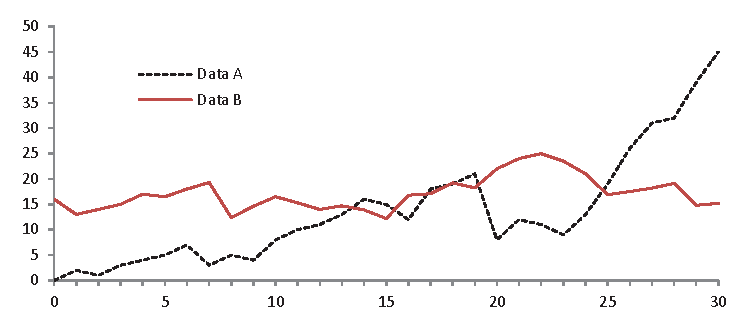
\includegraphics[width=\textwidth]{fig1.eps}
% \caption{A figure caption is always placed below the illustration.
% Please note that short captions are centered, while long ones are
% justified by the macro package automatically.} \label{fig1}
% \end{figure}

% \begin{theorem}
% This is a sample theorem. The run-in heading is set in bold, while
% the following text appears in italics. Definitions, lemmas,
% propositions, and corollaries are styled the same way.
% \end{theorem}
% %
% % the environments 'definition', 'lemma', 'proposition', 'corollary',
% % 'remark', and 'example' are defined in the LLNCS documentclass as well.
% %
% \begin{proof}
% Proofs, examples, and remarks have the initial word in italics,
% while the following text appears in normal font.
% \end{proof}
% For citations of references, we prefer the use of square brackets
% and consecutive numbers. Citations using labels or the author/year
% convention are also acceptable. The following bibliography provides
% a sample reference list with entries for journal
% articles~\cite{ref_article1}, an LNCS chapter~\cite{ref_lncs1}, a
% book~\cite{ref_book1}, proceedings without editors~\cite{ref_proc1},
% and a homepage~\cite{ref_url1}. Multiple citations are grouped
% \cite{ref_article1,ref_lncs1,ref_book1},
% \cite{ref_article1,ref_book1,ref_proc1,ref_url1}.
%
% ---- Bibliography ----
%
% BibTeX users should specify bibliography style 'splncs04'.
% References will then be sorted and formatted in the correct style.
%
% \bibliographystyle{splncs04}
% \bibliography{mybibliography}
%
\begin{thebibliography}{8}
\bibitem{ref_1}
memory-profiler 0.57.0, \url{https://pypi.org/project/memory-profiler/}. Last accessed 28 Feb 2020

\bibitem{ref_2}
S.J. Russel, P. Norvig: Artificial Intelligence: A Modern Approach. 3rd edn. Pearson, Harlow (1994)

\end{thebibliography}

\section{Appendices}
\subsection{Appendix A}

\begin{figure}
    \centering
    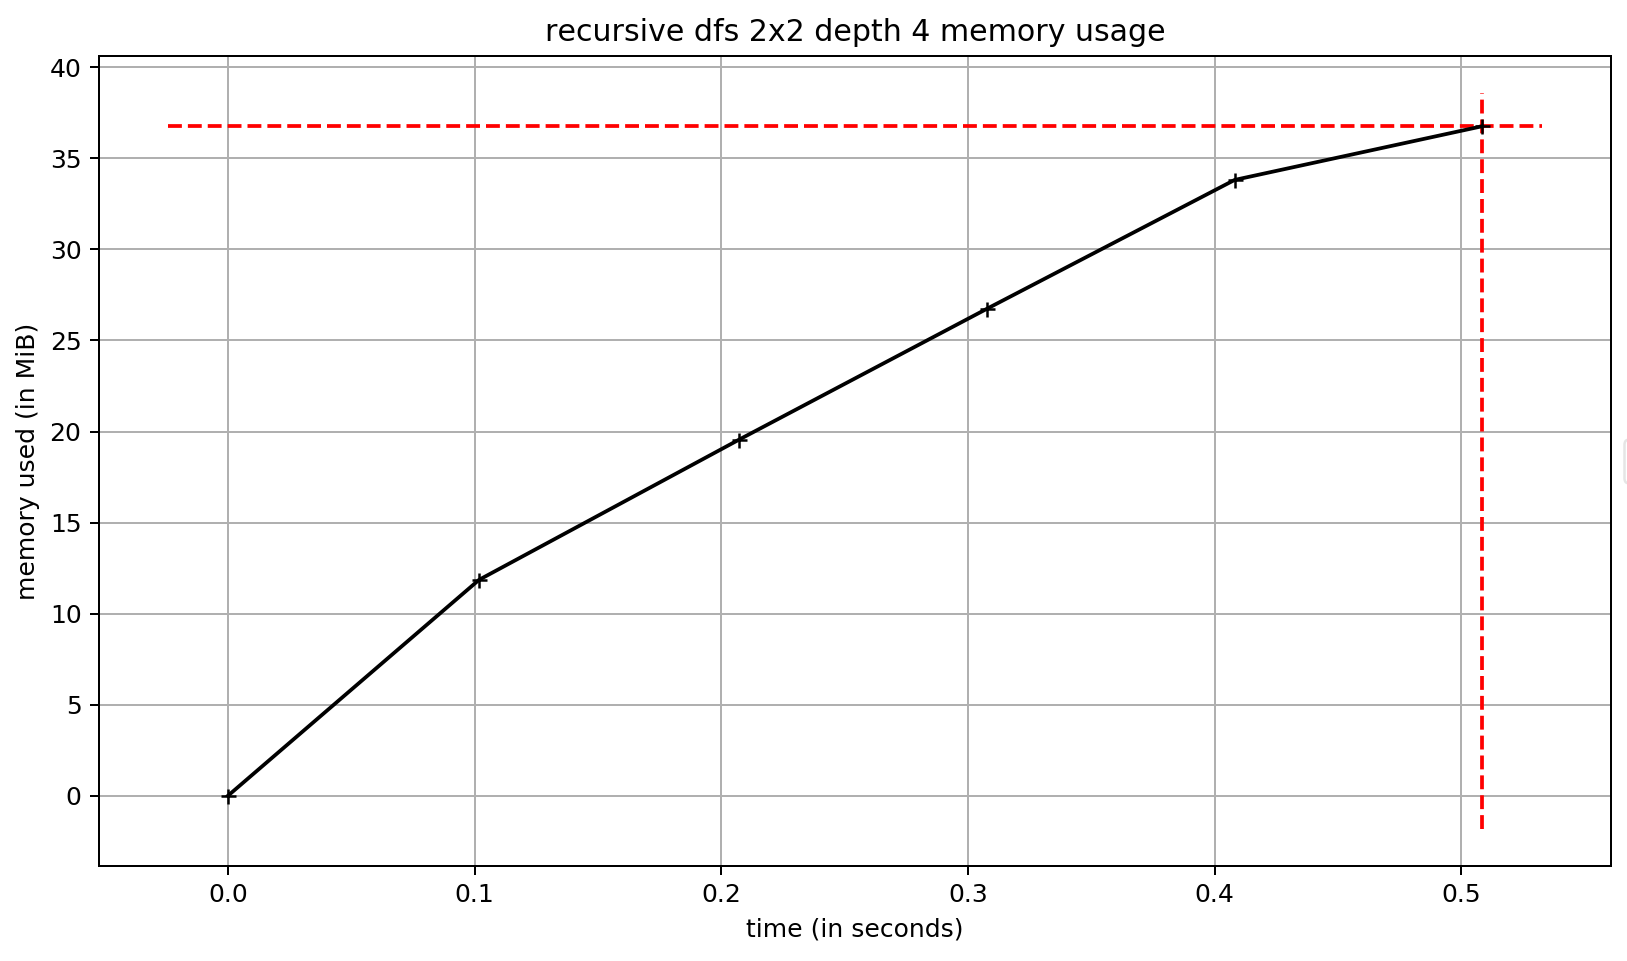
\includegraphics[width=9.5cm]{images/dfs-2x2.png}
    \caption{Memory usage of limited dfs on a 2x2 puzzle} \label{fig1}
    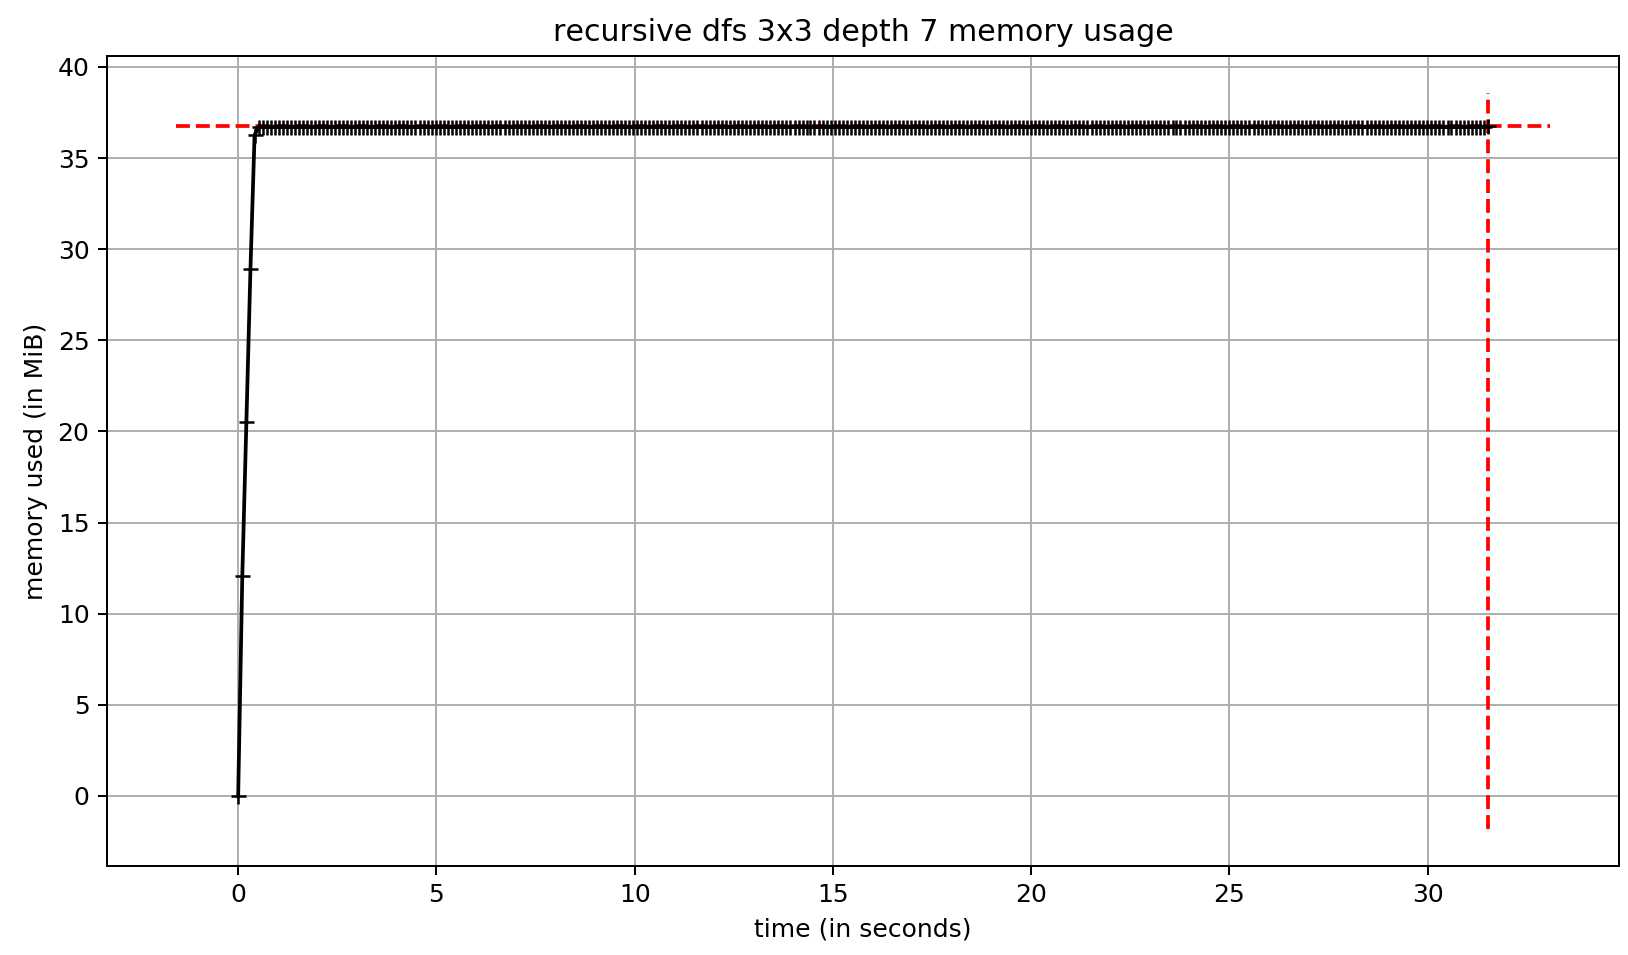
\includegraphics[width=9.5cm]{images/dfs-3x3.png}
    \caption{Memory usage of limited dfs on a 3x3 puzzle} \label{fig2}
    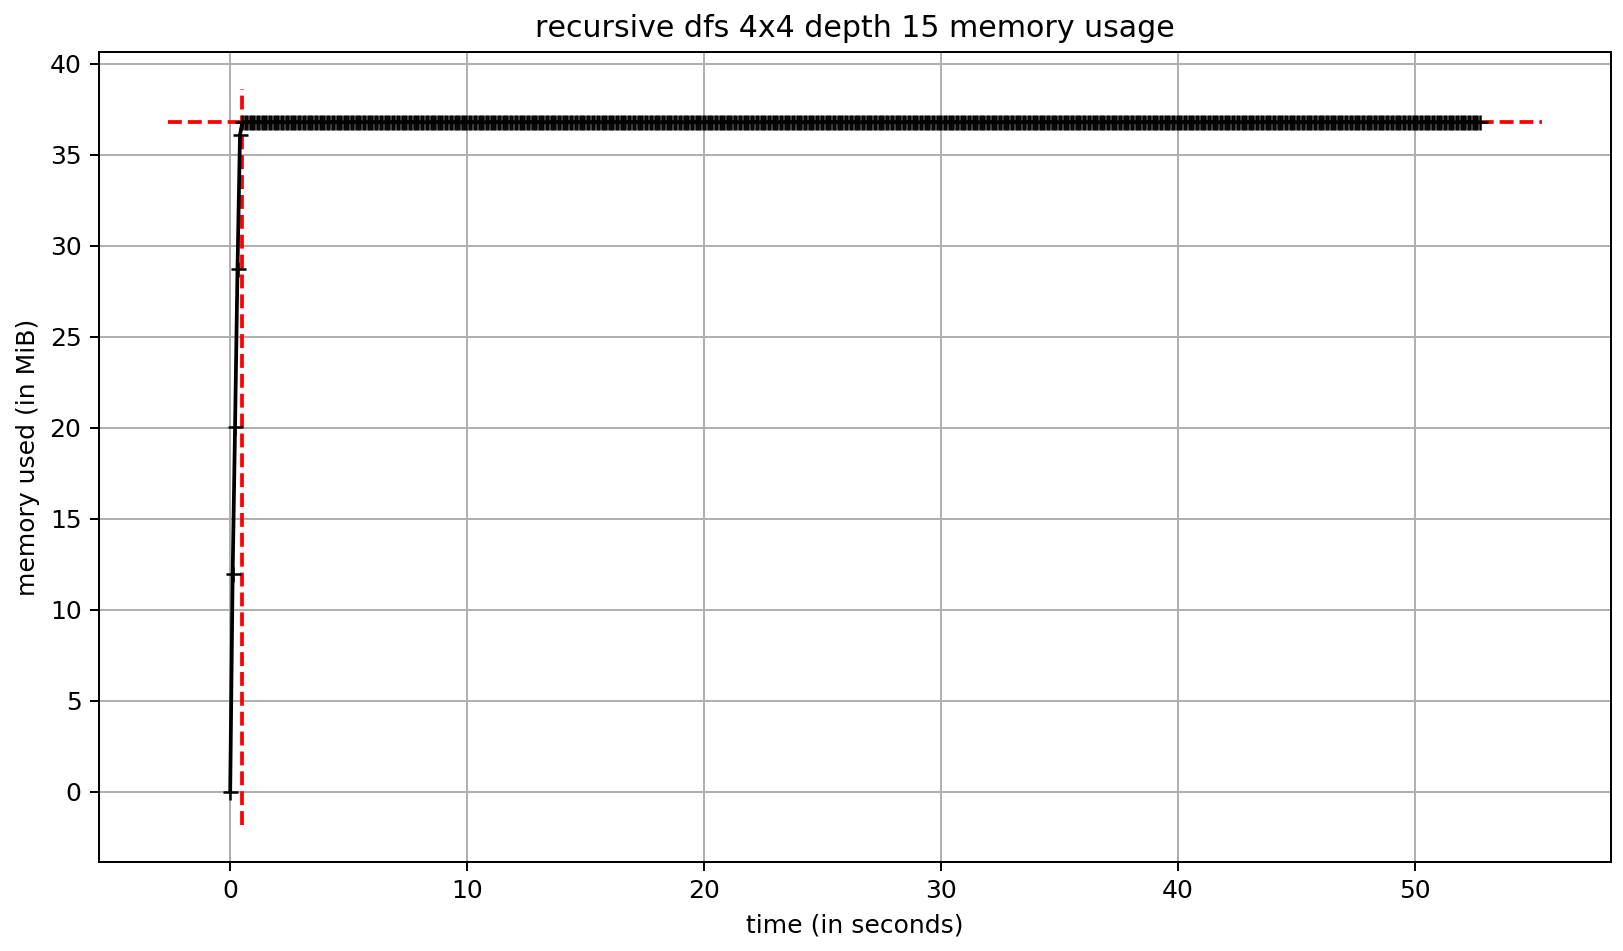
\includegraphics[width=9.5cm]{images/dfs-4x4.png}
    \caption{Memory usage of limited dfs on a 4x4 puzzle} \label{fig3}
\end{figure}

\end{document}

